%========================== main document start =======================%
\chapter{Individual Spread Footing}
\section{Introduction} Clause 34 of the  \citetitle{is4562000} gives the
provisions governing the design of reinforced concrete footings.  These
provisions are similar to those given by the \citeauthor{aci1981aci}. 
The design of footings in accordance with \citetitle{is4562000} differs
from that by the \citetitle{is4561964} in the following aspects.

\begin{enumerate}[I]
\item Perimeter shear stress must not exceed the allowable value. This
aspect was not given in the \citetitle{is4561964}. But it is similar to
the familiar concept of punching shear stress.

\item Bond-stress-criterion was given in the \citetitle{is4561964}, but it
is omitted in the \citetitle{is4562000}. Instead, development length of
footing bars is required to be checked at the sections where bending
moment is critical.

\item 25\% excess pressure on edge of footing was allowed by the 
\citetitle{is4561964} when a footing is eccentrically loaded. This 
concession is withdrawn by the \citetitle{is4562000}, thereby adding to 
the cost of eccentrically loaded footings.
\end{enumerate}
The \citetitle{is4562000} requires footings to be designed for 
the following limit states.

\begin{enumerate}[(a)]
\item Perimeter shear
\item Bending moment
\item Beam shear
\item Development length of footing bars
\item Development length of column bars
\end{enumerate}

\section{Types of Individual Footings} Individual spread footings can 
be either square or rectangular in plan, the area of a rectangular
footing with sides $A$ and $B$ being given by,

\begin{equation}
\label{eq:footingArea}
A \times B = \frac{P}{p}
\end{equation}
where $P$ is the column load in $\kn$ and $p$ denotes the net allowable
soil pressure in $\knpms$. In this development, self-weight of footing
may not be considered. This involves only a small error in that, the
weight of the concrete of footing is assumed here to be approximately
equal to the weight of the earth displaced by it. Further, it is assumed
here that the soil pressure under the footing is uniform. This is a 
reasonable assumption as discussed elsewhere. Various types of 
individual spread footings are shown in
\fig \ref{Types-of-individual-spread-footing}.
%---------------figures--------------------------%
\begin{figure}
\begin{subfigure}[b]{0.5\textwidth}
  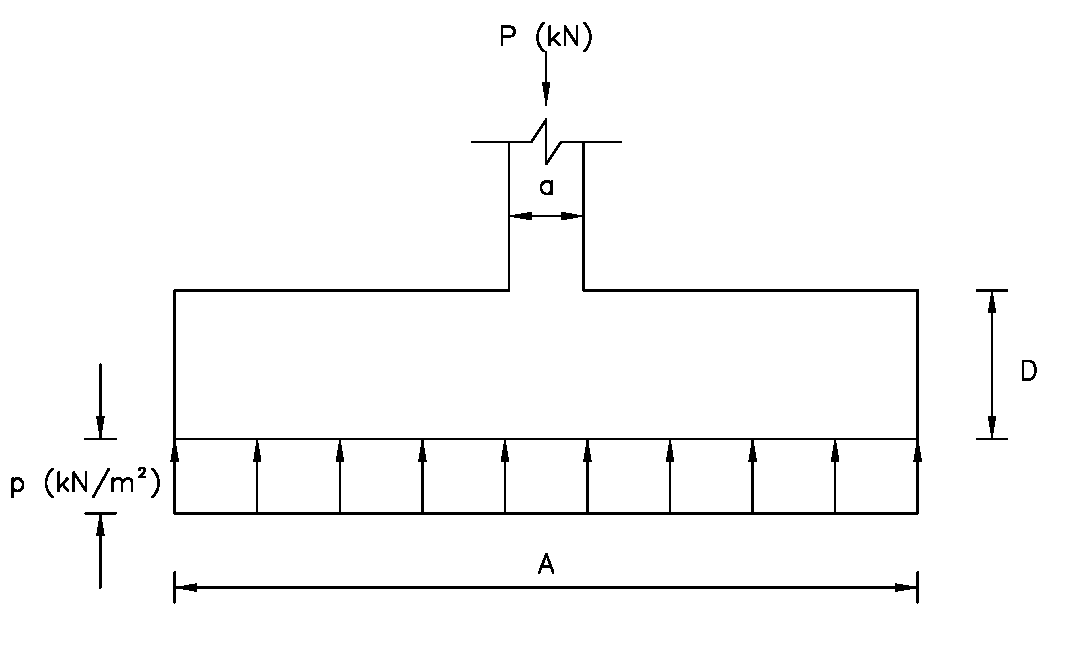
\includegraphics[width=\textwidth]{images/udf.pdf}
    \caption{Uniformly deep footing}
    \label{uniformdeepfooting}
  \end{subfigure}
  %
  \begin{subfigure}[b]{0.5\textwidth}
    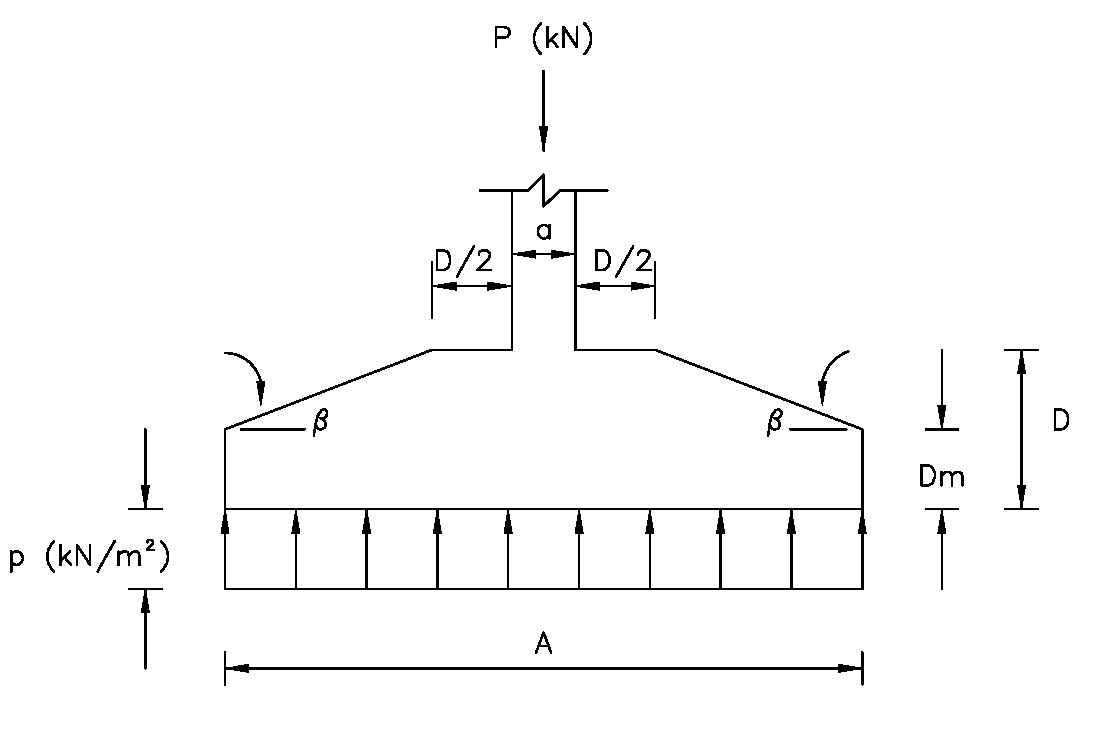
\includegraphics[width=\textwidth]{images/sfb.pdf}
    \caption{Sloped footing (slope starting from $D/2$ away from the
     edge of column)}
    \label{Slopedfooting}
  \end{subfigure}
 %
 \begin{subfigure}[b]{0.5\textwidth}
    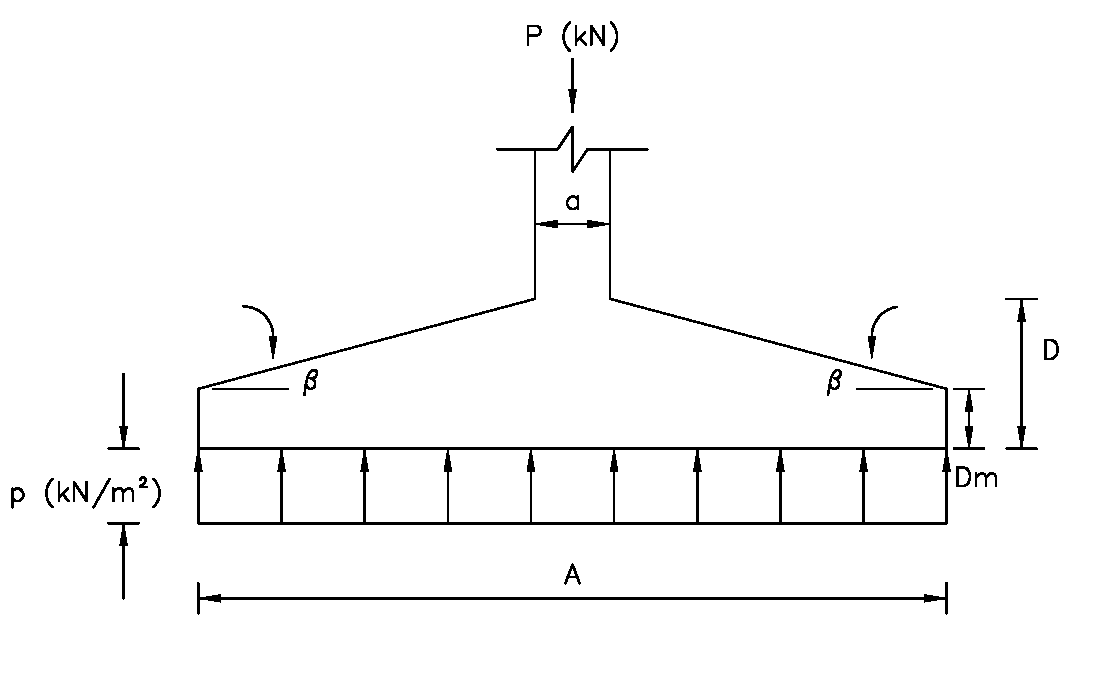
\includegraphics[width=\textwidth]{images/sfc.pdf}
    \caption{Sloped footing (slope starting from the edge of column)}
    \label{slopefooting}
  \end{subfigure}
 %
\begin{subfigure}[b]{0.5\textwidth}
    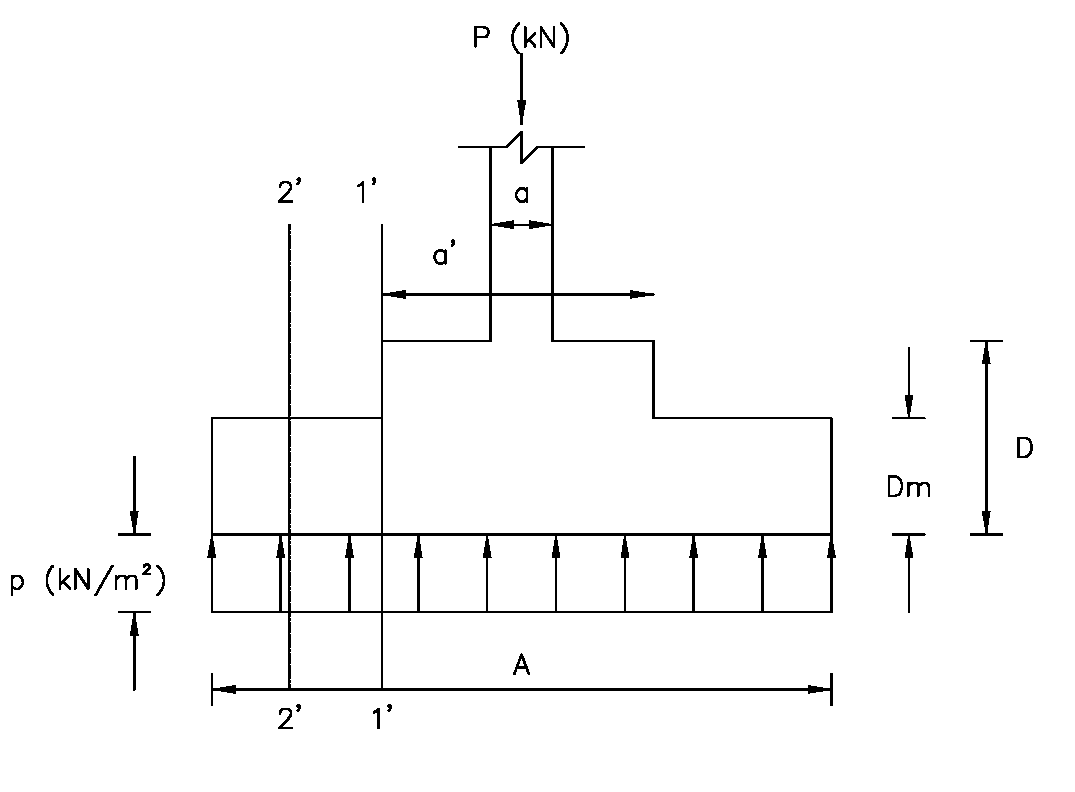
\includegraphics[width=\textwidth]{images/sfd.pdf}
    \caption{Stepped footing}
    \label{steppedfooting}
  \end{subfigure}
\caption{Types of individual spread footing.}
\label{Types-of-individual-spread-footing}
\end{figure}
%-----------------end figure-----------------------%
With the area of footing known from \eqn \ref{eq:footingArea},
dimensions $A$ and $B$ are easily finalise.  The only dimension of 
footing which remains to be known is the depth ($D$) of the footing.  
A common way of design of footing is to assume D, rather generously,
with a view to reduce steel area as well as to help provide fixity to
the column base, in order to be close to the assumptions made in the
frame analysis of superstructure.

\section{Design for Perimeter Shear} Depth of footing is fixed from 
the consideration of perimeter shear stress which depends on concrete
quality, being independent of types of reinforce steel. For a square 
footing of uniform depth with a square column of side $a$
(\fig \ref{critical perimeter 1-1-1-1}), perimeter shear stress
$\tau_{v}$ is given by

\begin{equation}
\label{eq:perimeterShearStress}
\tau_{v} = \frac{V_{u}} {{b_{0}} \times d} 
=\frac{1.5 \times S_{p}} {4(a + d) \times d} 
\end{equation}
where 
\begin{equation}
\label{eq:perimeterShearForce}
\quad S_{p} = P - p \times (a + d)^2
\end{equation}
and $b_0$ = Perimeter of critical closed section.

The allowable perimeter shear stress ${\tau_{a}}$ (clause 31.6.3 of
the \citetitle{is4562000}) is given by,

%------------------figures---------------------%

\begin{figure}
  \centering
  \begin{subfigure}[b]{0.5\textwidth}
    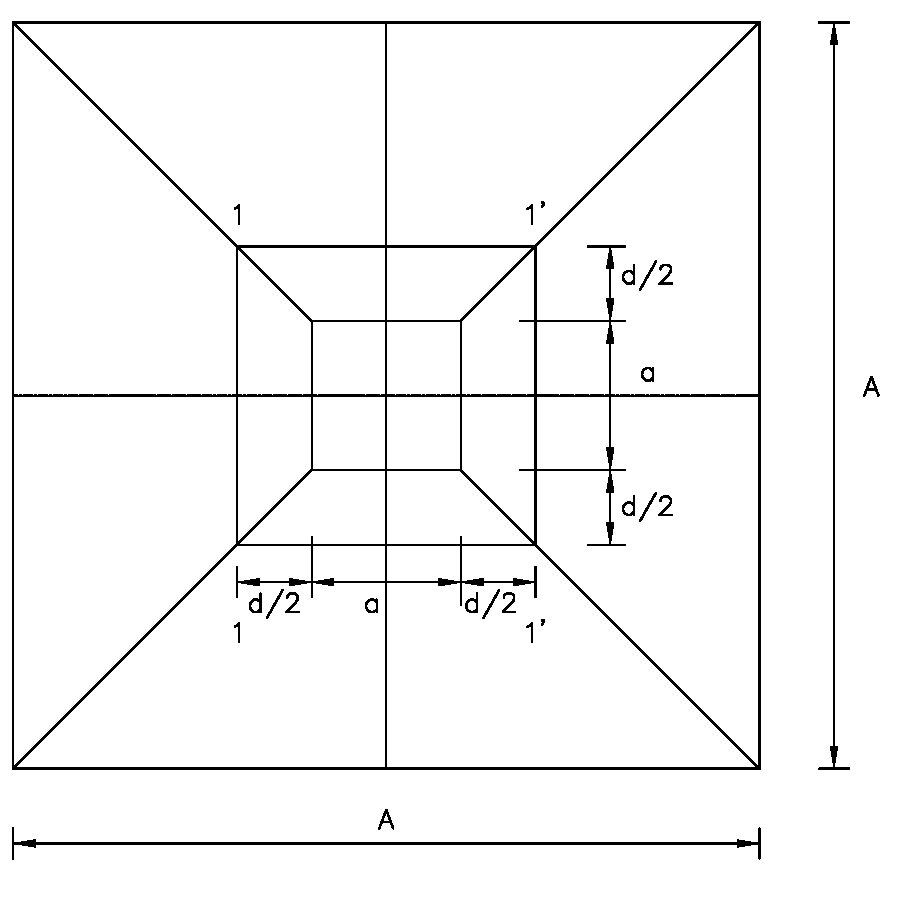
\includegraphics[width=\textwidth]{images/cp.pdf}
    \caption{Critical perimeter 1-1-1-1 in plan for perimeter shear}
    \label{critical perimeter 1-1-1-1}
  \end{subfigure}\\
  %
  \begin{subfigure}[b]{0.5\textwidth}
    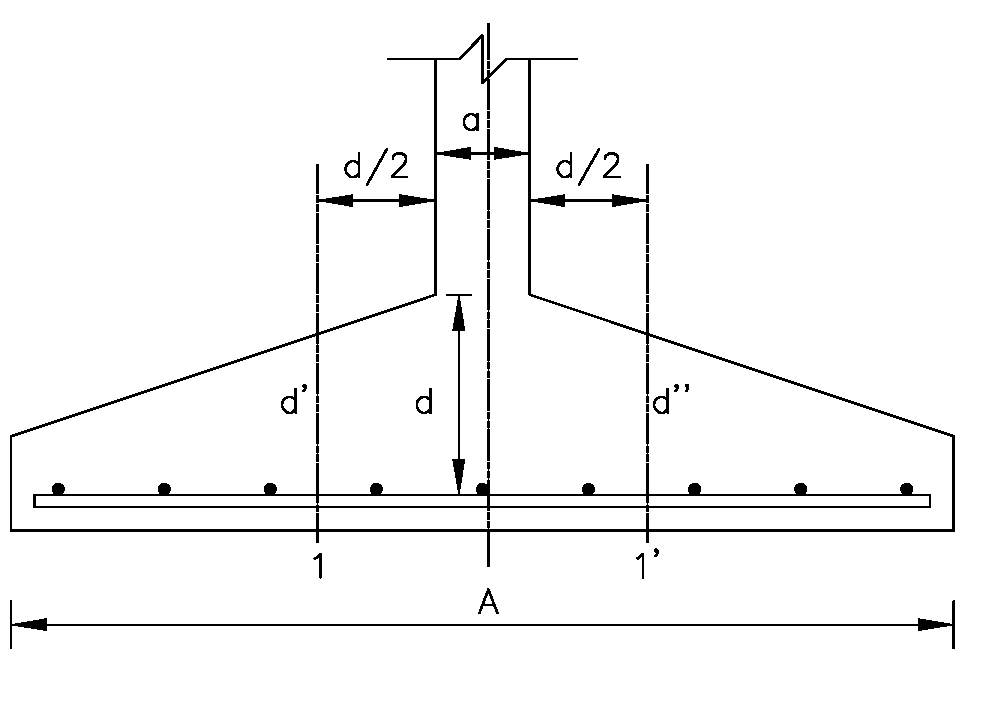
\includegraphics[width=\textwidth]{images/sh.pdf}
    \caption{Section of sloped footing showing reduced depth ${d'}$
     for perimeter shear}
    \label{sectionslopefooting}
  \end{subfigure}
\caption{Perimeter shear for square footing.}
\label{Perimeter-shear-for-square-footing}
\end{figure}

%------------------end figure---------------%

\begin{equation}
\label{eq:allowable2DShearStress}
\tau_{a} = k_{s} . \tau_{c} = k_{s} \times 0.25 \sqrt{f_{ck}}
\end{equation}
where, $f_{ck}$ is to be put in $\npmms$.

$k_{s}$ = 1.0 for square columns and also for rectangular with aspect 
ratio $\left( \dfrac{b}{a} \right) \leq {2.0}$. For the condition 
$\tau_{v} = \tau_{a}$, \eqn (\ref{eq:perimeterShearStress}) and
(\ref{eq:allowable2DShearStress}) give,

\begin{sagesilent}
  var('a,A,d,fck,p,k,consst,alpha')
  consst = .067
  consst = consst.n(digits=3)
  z1=(1-(a/A)**2-2*(a/A)*(d/A)-(d/A)**2)/((a/A)*(d/A)+(d/A)**2)
  z2=(consst*fck**(1/2)*alpha)/p
\end{sagesilent}

\begin{equation}
  \label{eq:areafck}
  \sage{z1}=\sage{z2}=\sage{k} (say)
\end{equation}
For a square sloped footing with a square column of side $a$
(\fig \ref{sectionslopefooting}),
 
\begin{equation}
\label{eq:shearSquare}
\tau_{v} = \frac{V_{u}}{b_{0} \times d''}
=\frac{1.5 \times {S_p}}{4(a + d) \times d''}
\end{equation}
Assuming $d''$ = $ \alpha . d $, the condition $\tau_{v} = \tau_{a}$
 gives,

\begin{equation} 
 \label{eq:areafckSloped}
  \sage{z1}=\sage{z2}=\sage{k}                                   
\end{equation} 
$\alpha = 1.0$ for footings of Types ($a$), ($b$) and ($d$) 
(\fig \ref{Types-of-individual-spread-footing}),
while $\alpha$ $<$ 1.0 for sloped footings of Type ($c$). The overall
depth of footing is given by,

\begin{sagesilent}
  var('D,d,c,phi')
  z=d+c+phi
\end{sagesilent}

\begin{equation}
  \label{eq:depth-cover}
  \sage{D}=\sage{z}
\end{equation}
Here, $d$ is regarded as an average value for either steel layer. For
sloped footings  (\fig \ref{sectionslopefooting}), simple geometry
gives,

\begin{equation}
\label{eq:shape}
\alpha = \frac{d''}{d} = \frac{{D_m}}{d} + \frac{D - {D_m}}{d}.
\frac{\left(1 - \dfrac{a}{A} - \dfrac{d}{A}\right)}
{\left(1 - \dfrac{a}{A}\right)}=\dfrac{(c+\phi)}{d}
\end{equation}
\chartm \ref{Dummy chart} is developed on the basis of
\eqn (\ref{eq:areafck}) and (\ref{eq:areafckSloped}) and it
applies to both uniformly deep and sloped square footings. It can also
be used for rectangular footings with rectangular columns by using 
average values of $a$ and $A$, provided an equal overhang is left on
all sides of column, which requires,

\begin{sagesilent}                                                      
        var('b,a,B,A')                                                
        z=b-a
        z2=B-A                                                   
\end{sagesilent}

\begin{equation}
  \label{eq:equaloverhang}
           \sage{z}=\sage{z2} 
\end{equation}
Solution of numerical examples gives an idea that it is possible to
develop thumb rules for fixing depth of footings. It may be noted that
there is no dire need of exactness in fixing the value of depth of
footing, only it should be more than adequate for the actions imposed
on a footing. \tablem \ref{chaptertable}, based on
\eqn (\ref{eq:areafck}), is developed for footings of Types ($a$) 
and ($b$) (\fig \ref{Types-of-individual-spread-footing}).It gives
values of $D/A$ for various practicable values of $p$. It is seen that,
for safety in beam shear, these values are to be increased by 10\% in 
case of steel types \fefouronefive and \fefivezerozero. For 
sloped and stepped footings (Types $c$ and $d$), the depth of footing 
given by \tablem \ref{chaptertable} may be increased by 20\%. The
depth at the free end of a footing may be restricted to 150 mm, which 
is the minimum prescribed by the ~\citetitle{is4562000} for spread
footings.
 

%%==================  End of My correction  ========================%


\section{Design for Moment and Beam Shear} 
Section 1-1 in \fig \ref{critical-sections-for-bending-moment-and-beam-shear-in-footing} 
is the critical  section for bending moment.
The bending moment for full width $B$ is given by,

\begin{sagesilent}                                                      
        var('p,B,A,a,k,N,mm')                                                
        z=(p*B*(A-a))/8                                           
\end{sagesilent}  

\begin{equation}
        \label{eq:criticalMoment}
        M_{1-1}=\sage{z}
\end{equation}
For footings of uniform depth and also stepped footings, the concrete
compression zone is rectangular and charts of Chapter 2 are used to 
calculate the required area of steel. But for slopped footings, the 
concrete compression zone is of a trapezoidal shape and \chartm 
$4.1$ of Chapter $4$ is to be used for finding steel area. \chartm 
4.1 can be used for both uniformly deep $(\gamma = 0)$ and sloped
footings. The calculated steel area should not be less than the 
specified minimum steel area (\tablem 11.4 of Chapter 11) for spread
footings which may be regarded as slabs for this purpose.

Section 2-2 in \fig \ref{critical-sections-for-bending-moment-and-beam-shear-in-footing}
is the critical section for beam shear. The shear force and moment at
section ${2'-2'}$ for the full width of footing is given by,

\begin{sagesilent}
var('p,B,b,A,a,d')                                                
z=(p*B)*((A-a)/2-d)                                                      
z2=(p*(B/2))*(((A-a)/2)-d)**2
\end{sagesilent}  

\begin{equation}
      \label{eq:shear22}   
         S_{2-2}=\sage{z}
\end{equation}

\begin{equation}
        \label{eq:moment22}
        M_{2-2}=\sage{z2}
\end{equation}

\begin{sagesilent}
        var('tau_v,V_u')
        z=V_u/(b*d)
\end{sagesilent}
%-------------------figure------------------------%

\begin{figure}
  \centering
  \begin{subfigure}[b]{0.5\textwidth}
    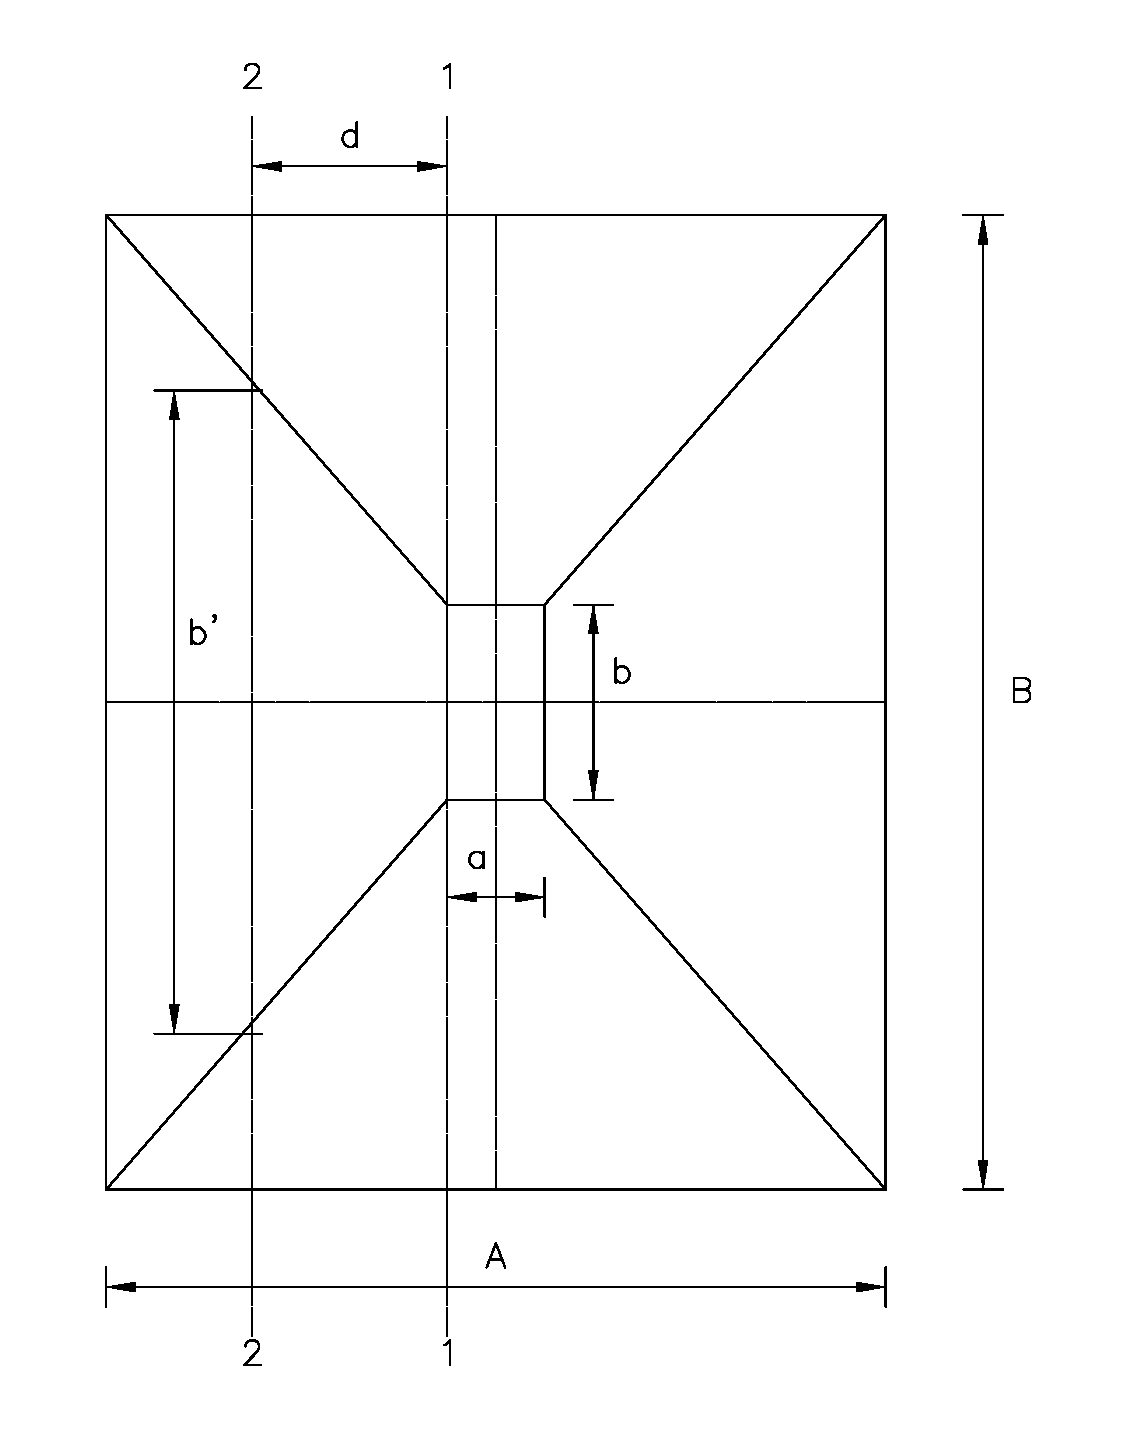
\includegraphics[width=\textwidth]{images/criticalsection(a).pdf}
    \caption{Plan of sloped footing}
    \label{Planofslopedfooting}
  \end{subfigure}\\
  %
  \begin{subfigure}[b]{0.5\textwidth}
    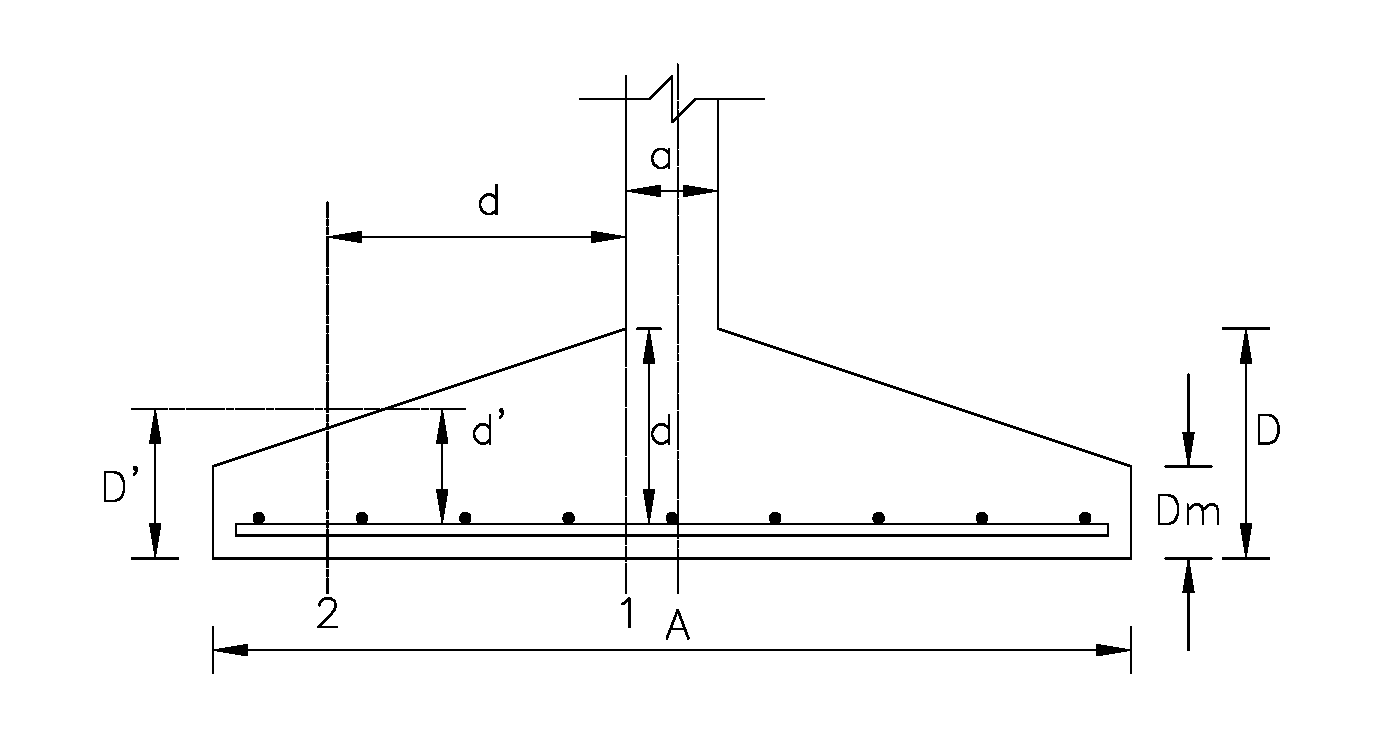
\includegraphics[width=\textwidth]{images/criticalsection(b).pdf}
    \caption{Section of sloped footing}
    \label{sectionofslopedfooting}
  \end{subfigure}
\caption{Critical sections for bending moment and beam shear in 
footings.}
\label{critical-sections-for-bending-moment-and-beam-shear-in-footing}
\end{figure}
%--------------------end figure-------------------%
Beam shear stress $\sage{tau_v}$ for footings of uniform depth and 
stepped footings is given by,

\begin{equation}
         \label{eq:shearstress22}
        \sage{tau_v}=\sage{z}= \frac{{1.5} \times S_{2-2}}{bd}
\end{equation}
where, $$b = \text{B for uniformaly deep footings,}$$ 
$$= \text{a for stepped footing} (\fig \ref{steppedfooting})$$
For sloped footings, clause 40.1.1 of the  \citetitle{is4562000} gives,
(-ve sign applies here),

\begin{equation}
         \label{eq:clause40.1.1}
        \sage{tau_v}=\frac{\quad{V_u}}{b'd'}-\frac{M_u}{b'd'^2}.tan\beta
\end{equation}
where b', d' are shown in \fig \ref{Planofslopedfooting} and 
\fig \ref{sectionofslopedfooting} and ${M_u}$ is the ultimate
moment at section 2-2.

\begin{sagesilent}
        var('D_m,D,a,A,d')
        z=D_m+((D-D_m)*(1-(a/A)-2*(d/A))/(1-(a/A)))
        var('phi,c')
        z2=c+phi
        var('b,B')
        z3=b+2*((B-b)/(A-a))*d
        be=var('beta')
        z4=tan(be)
        z5=2*((D-D_m)/(A-a))
        z6=2*(D-D_m)/(A-a-D)
\end{sagesilent}
\begin{equation}
        \label{eq:ultimatemoment22}
        D'=\sage{z}
\end{equation}

\begin{equation}
         \label{eq:ultimatemoment22b}
        d'=D'-(\sage{z2})
\end{equation}

\begin{equation}
         \label{eq:ultimatemoment22c}
        b'=\sage{z3} \sage{be}
\end{equation}

For Type (c), \fig \ref{slopefooting} gives,
\begin{equation}
         \label{eq:12.19}
        \sage{z4}=\sage{z5}
\end{equation}


For Type (b), \fig \ref{Slopedfooting} gives,
\begin{equation}
         \label{eq:12.20}
        \sage{z4}=\sage{z6}
\end{equation}

\begin{sagesilent}
        var('k,tau_a,tau_v,tau_c')
        z=k*tau_c
        var('V_v')
        z2=V_v/(b*d)
\end{sagesilent}
The calculated value of $\sage{tau_v}$ must not exceed the allowable 
stress $\sage{tau_a}$, as shear reinforcement is just not provided in
individual footings for reasons of economy, the same as in solid slabs.
The allowable stress in concrete solid slabs $\sage{tau_a}$ is given by,

\begin{equation}
         \label{eq:concretesolidslabs}
        \sage{tau_a}=\sage{z}
\end{equation}
$\sage{tau_c}$ is given by \tablem 19 of the  \citetitle{is4562000} 
depending on the steel area provided for moment at the critical section
2-2 (the minimum value of $\sage{tau_c}$ is assumed for 
$p_t $$\leq$$ 0.15$ in \tablem 19 and

$$\begin{array}{l@{}l}
&{}k=1.0 \text{ for } D \geq 300 \mm\\
&{}=1.1 \text{ for } D = 250 \mm\\   
&{}=1.2 \text{ for } D = 200 \mm\\
&{}=1.25 \text{ for } D = 175 \mm\\   
&{}=1.30 \text{ for } D \leq 150 \mm
\end{array}$$
Normally, depth of footing given for perimeter shear
(\chartm \ref{Dummy chart}) is more than adequate
to satisfy the requirements of beam shear. But when steel type 
{\fefouronefive} and {\fefivezerozero} are used as reinforcement
beam shear may govern the depth of footing. For stepped footings,
additional checks for moment and beam shear are required to be made for
the portion of the footing of depth $D_m$ (\fig \ref{steppedfooting}).
When section ${1'-1'}$ is the critical section for moment and section
${2'-2'}$ is that for beam shear (\fig \ref{steppedfooting}), 
expressions for moment and shear are given as,

\begin{equation}
         \label{eq:momentandshear1-1}
        M_{1'-1'}=p.B.\frac{(A-a')^2}{B}
\end{equation}

\begin{equation}                                             \label{eq:momentandshear2-2}
        S_{2'-2'}=p.B\bigg[\frac{(A-a')^2}{B}-d_m\bigg]                                 
\end{equation}
For finding steel area, \chartm 4.1 (with $\gamma = 0$), may be used,
as the concrete compression zone is of a rectangular shape of width equal 
to B. Shear stress $\tau_v$ is given by,

\begin{equation}
        \label{eq:Shearstress}
        \sage{tau_v}=\sage{z2}=\frac{1.5S_{2-2}}{B.d_m}
\end{equation}
and it must not exceed $\tau_a$ given by \eqn (\ref{eq:concretesolidslabs}),
failing which depth $D_m$ should be suitably increased. Normally
$D_m = 0.30$ $D$ to $0.50$ $D$ is kept in stepped footings and perimeter 
shear stress can be checked to be safe by using first principles.

%------------------figure-------------------------------%
\begin{figure}
  \centering
  \begin{subfigure}[b]{0.5\textwidth}
    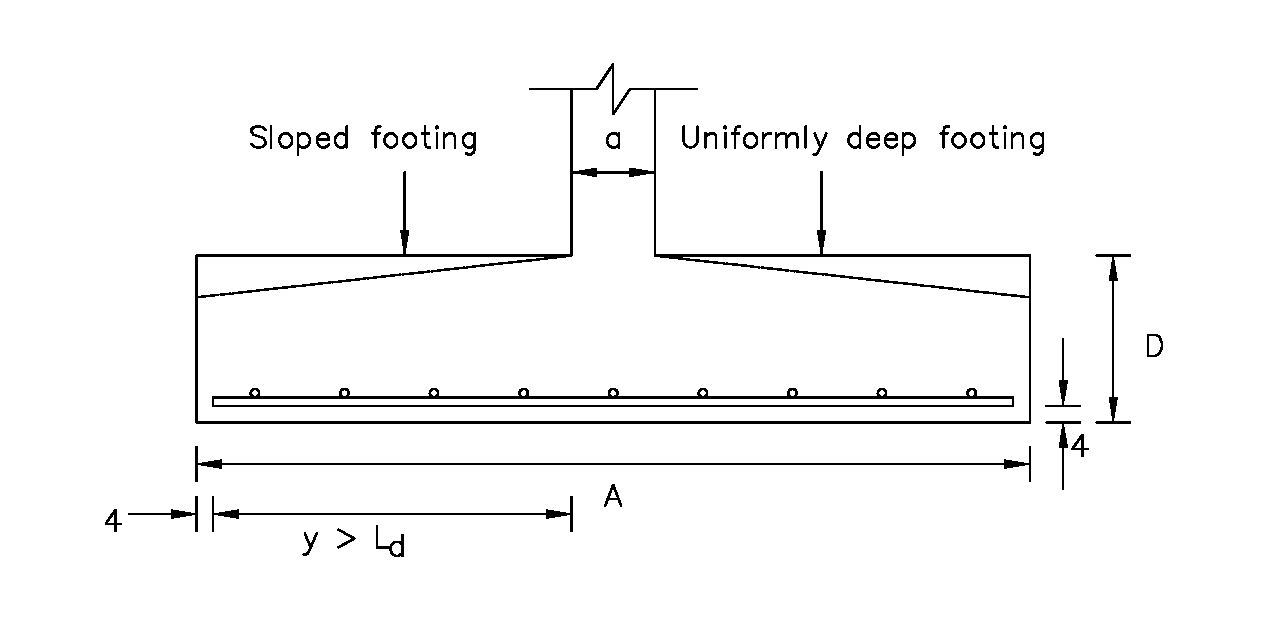
\includegraphics[width=\textwidth]{images/developmentlength(a).pdf}
    \caption{Section of uniformaly and sloped footing}
    \label{uniformallydeepfooting}
  \end{subfigure}\\
  %
  \begin{subfigure}[b]{0.5\textwidth}
    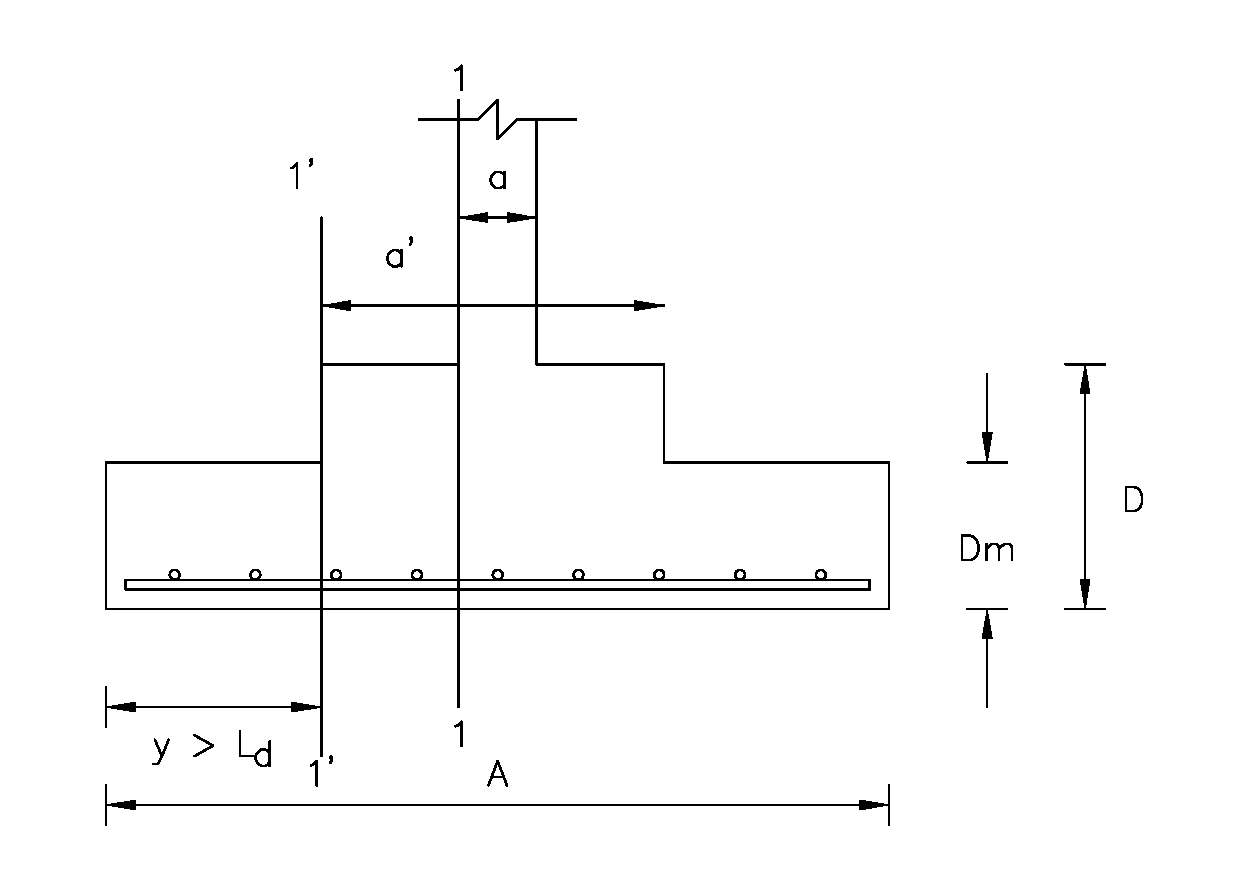
\includegraphics[width=\textwidth]{images/developmentlength(b).pdf}
    \caption{Section of stepped footing}
    \label{stepedfoting}
  \end{subfigure}
\caption{Development length of footing bars.}
\end{figure}

%------------------end figure---------------------------%
\section{Development Length of Bars}
Column dowel bars should extend into footings for a distance equal to 
the development length (\tablem 11.3 of Chapter 11) of column bars
in compression (or in tension when moment in column is large). With the
clause 26.2.2.2 of the \citetitle{is4562000}, column bars can always be adequately
anchored in the footing, whatever be the depth of footing. 

\begin{sagesilent}
        z=((A-a)/2)-4                    
\end{sagesilent}

For development length of footing bars, there should be adequate bar
length available $(y)$, either straight or bent-up or both measured from
the face of column. Referring to \fig\ref{uniformallydeepfooting},
for sloped or uniformly deep footings,

\begin{equation} 
        \label{eq:uniformallydeepfooting}
        y= \sage{z} >L_d (tension)
\end{equation}
where 40 $\mm$ is taken as clear cover over ends of bars in footings. If 
\eqn \ref{eq:uniformallydeepfooting} is not  satisfied, there are
two ways to tackle this problem :

\begin{enumerate}
\item bend bars up, as shown dotted in \fig \ref{uniformallydeepfooting}
\item choose smaller diameter for bars.
\end{enumerate}

For stepped footings \fig \ref{stepedfoting}, the available
straight length of bars beyond the critical section ${1' - 1'}$ is,
                                                          
\begin{equation}                            
       \label{eq:criticalsection1-1}
        y'= \frac{(A-a')}{2}-4 >L_d (tension)                                      
\end{equation}
Normally, full steel area required at section $1 — 1$ is provided 
throughout and the steel strength $\sigma_s$ at section 1’ - 1’ may be
less than its maximum value of 0.87 $f_y$. The value of $L_d$ (tension)
should be calculated for the appropriate value of $\sigma_s$.

\section{Selection of Type of Footings}
Footings of uniform depth (Type $a$), though commonly used in practice
for reasons of ease in design and construction, are the costliest. These
consume more concrete quantity (about 25\% to 45\%) than that by sloped
footings. This type is suitable only for small footings with overall
depth being restricted to, say, 300 $\mm$.

For footings of intermediate size, sloped footings with slope starting
from $\dfrac{D}{2}$ away from the edge of column (Type $b$), are quite 
suitable. This type is quite economical giving concrete and steel 
quantities quite reasonable in comparison with other types. This type 
is easy to design as well as to execute. This type is recommended for
most individual footings encountered in buildings with overall depth
greater than 300 $\mm$. The depth at the free end of footing may be kept 
at 150 $\mm$, the specified minimum given by the \citetitle{is4562000}. The depth ($D$) of
this type of footing is kept the same as that for footings of uniform
depth.

For large-sized footings, sloped footings with the slope starting from 
the edge of column (Type $c$) or stepped footings (Type $d$) are
preferred to other types, as these give the least quantities for
concrete and steel consumption. The stepped footings give the least
steel quantity, while the sloped footings (Type $c$), give the least
concrete quantity. The depth for these types of footings works out to
be about 20\% more than that for footings of uniform depth. Stepped
footings are a little cumbersome in construction, while the sloped 
footings are easier in execution, albeit a little more labour-intensive 
than the footings of uniform depth.

%====================== first numerical example ======================%

\section{Examples}
\begin{example}
Square footing of Uniform Depth (Type a).\\
\given
\begin{sagesilent}
  var('PP,pp,aa,ff_ck,ff_y')
  PP = 1000
  pp = 200
  aa = 400
  ff_ck = 15
  ff_y = 415
\end{sagesilent}

$$P = \sage{PP} \kn$$
$$p = \sage{pp.n(digits=1)} \knpms$$
$$a = \sage{aa} \mm$$
$$f_{ck} = \sage{ff_ck} \npmms$$
$$f_y = \sage{ff_y} \npmms$$
\required Design the footing\\
\solution

\begin{enumerate}[(i)]
\item \textbf{Dimensions of footing}\\

\begin{sagesilent}                                                      
def multipleCheck(number, divisor=25):                                
# If not directly divisible by divisor.                                 
  if (number % divisor) != 0:                                             
      y = int(number / divisor)   # flooring the value.             
      y += 1                      # Adding 1 for choosing next multiple.
      final_value = y * divisor   # Multiply the new quotient with divisor.
                                                                        
  elif number == 0:                                                     
      final_value = divisor                                             
                                                                        
  else:                                                                 
      final_value = number                                              
  return final_value                                                     
\end{sagesilent}        

\begin{sagesilent}
  var('A,P,p')
  
  pp = pp/1000000.n(digits=2)

  f(P,p)=P/p
  A(P,p)=(f(P,p))^(1/2)
  
  s0=f(P,p)
  s=f(PP,pp)
  o1=A(PP,pp).n(digits=4)
  s1=multipleCheck(o1)
\end{sagesilent}

\eqn \ref{eq:footingArea} gives, 

$$A^2 = \sage{s0} = \sage{s.n(digits=5)} \mms$$
$$A = \sage{o1} \mm$$
$$A = \sage{s1} \mm$$

\begin{sagesilent}
  p(A)=1000/(A*A)
  s2=p(s1)
  s2 = s2*1000000.n(digits=4)
\end{sagesilent}

Provided $\sage{s1} \times \sage{s1}$ base and  
$$p = \sage{s2} \knpms$$

\begin{sagesilent}
  var('AA,const')
  const = 4.5
  f1(AA) = AA/const.n(digits=3)
  s3=f1(A)                                           
  s4=f1(s1) 
\end{sagesilent}

\tablem \ref{chaptertable} gives for $p = \sage{pp.n(digits=2)}$, 
and steel \fefouronefive,
 
$$D = \sage{f1(A)} = \sage{s4} \mm$$   


\begin{sagesilent}
  var('alpha')
  f2(f_ck,alpha,p)=(10000*.067.n(digits=2)*((f_ck)^(1/2))*alpha)/(p)
  s5=f2(f_ck,alpha,p)
  s66=f2(ff_ck,1,s2)
  
  f3(a,A)=a/A
  s6=f3(a,A)
  s7=f3(aa,s1).n(digits=3)

  f4(A,q)=q*A
  s8=f4(A,s7)
  s9=f4(s1,s7)

  e1(a,k) =1/(-1/2*(a*k + 2*a - sqrt(a^2*k^2 + 4*k + 4))/(k + 1))          
  o2 = e1(a,k)                                                          
  o3 = e1(s7,s66) 
  o4 = o3.n(digits=2) 
  
  s9 = f4(s1,o4)
  o9 = s9.n(digits=3)

  e3(A,o) = A/o
  o7 = e3(A,o4)
  s9 = e3(s1,o4)

  o5 = f3(A,d)
\end{sagesilent}

\item \textbf{Check for perimeter shear}   

\chartm \ref{Dummy chart} gives for, 

$$k = \sage{s5} = \sage{s66.n(digits=4)}$$
$$\sage{s6} = \sage{s7}$$

$$\sage{o5} = \sage{o4}$$

$$d = \sage{s9}$$ 

\begin{sagesilent}
  var('cc,pphi')
  cc=40
  pphi=12
  f5(d,c,phi) = d + c + phi
  s10 = f5(d,c,phi)
  s11 = f5(s9,cc,pphi)
  s11 = s11.n(digits=4)
  s107= s11.n(digits=4)  
  s11=multipleCheck(s11,25)
  s11 = s11.n(digits=4) 
 
  f6(p,B,A,a) = p*B*((A-a)^2)/8
  s12 = f6(p,B,A,a)
  s13 = f6(s2,s1/1000,s1/1000,aa/1000)

  f7(D,c,phi) = D-c-phi
  s14=f7(D,c,phi)
  s15=f7(s11,cc,pphi)

  f8(M_1,A,d) = ((10^5)*1.5*M_1)/(1.5*A*(d**2))
  s16=f8(M_1,A,d)
  s17=f8(s13,s1,s15)
  
  if(s4>s107):
    s109 = multipleCheck(s4)
  else:
    s109 = multipleCheck(s107)
\end{sagesilent}

\eqn \ref{eq:depth-cover} gives with $c = \sage{cc.n(digits=2)} \mm,
\phi=\sage{pphi.n(digits=2)}$,
$$D = \sage{s10} = \sage{s107} \mm$$
$$D = \sage{s109} \mm \text{ is safe} $$

\item  \textbf{Design for moment}  
\eqn \ref{eq:criticalMoment} gives,

$$M_{1-1} = \sage{s12} = \sage{s13.n(digits=4)} \knm$$

With rectangular compression zone, \chartm (2.2) gives for,   
$$d = \sage{s14} = \sage{s15.n(digits=4)}\mm$$
$$k = \sage{s17.n(digits=4)}$$
\begin{sagesilent}
  var('mu')
  
  # f9(mu)=mu/.87
  #mu=.0475
  #s20=f9(mu)

  f9(mu,A,d,f_ck,f_y)=(mu*A*d*f_ck)/(.87.n(digits=3)*f_y)
  s18=f9(mu,A,d,f_ck,f_y)
  mu = .0475

  s19=f9(mu,s1,s15,ff_ck,ff_y).n(digits=4)

  f10(A_st,A)=A_st/A
  s20=f10(A_st,A)
  
  s21=s1/1000
  s22=f10(s19,s21)
  
  f11(D) = 1.2.n(digits=2)*D
  s23=f11(D)
  #s24=f11(s11)
  s24 = f11(s109)

  d1= (1000)/(120)
  d3=d1.n(digits=0)
  w1(d4,r) = (d4*3.14*r**2)/100
  d2=w1(d3,6)
  d2 = d2.n(digits=2)

  if(s22>s24):
    q299 = s22
  else:
    q299 = s24


  diaa = 12
  m300(dia,qqq) = (3.14*1000*((dia)^2))/(qqq*4)                              
  q300 = m300(dia,qqq)                                                  
  q301 = m300(diaa,q299)                                                
  q301 = int(q301)                                                      
                                                                       
  m301(dia,qqq) = (3.14*1000*((dia)^2)*1)/(4*qqq)                            
  q302 = m301(dia,qqq)                                                  
  q303 = m301(diaa,q301).n(digits=4)  
  d2 = q303

\end{sagesilent}
$$\mu = \sage{mu.n(digits=2)}$$
$$A_{st} = \sage{s18} = \sage{s19} \mms$$

$$\sage{s20} = \sage{s22} \mmspm$$
 
\tablem 11.4 gives the minimum tension steel area in footings taken
as slab,

$$A_{st}(min) = \sage{s23} = \sage{s24} \mmspm$$

$\phi 12/\sage{q301}$ $c/c$ both ways provided giving an area$ = \sage{q303} \mmspm$\\ 
which is exceeded by that provided. 

\item  \textbf{Design for beam shear}\\                              
          \eqn \ref{eq:shear22} gives, 

\begin{sagesilent}
  f12(p,A,a,d)=p*A*(((A-a)/2)-d)
  s25=f12(p,A,a,d)
  s26=f12(s2,s1/1000,aa/1000,s15/1000)

  f13(S_22,A,d) = (1.5.n(digits=2)*S_22)/(A*d)
  s27 = f13(S_22,A,d)
  s28 = f13(s26,s1,s15)*1000
  
  f14(A_s,b,d) = (100 * A_s)/(b*d)
  s29 = f14(A_s,b,d)
  s30 = f14(d2,1000,s15)
\end{sagesilent}

$$S_{2-2} = \sage{s25} =\sage{s26.n(digits=4)} \kn$$
\eqn \ref{eq:shearstress22} gives

$$\tau_{v} = \sage{s27} = \sage{s28} \npmms$$

$$\sage{s29} = \sage{s30}$$
        
Table 19 of the \citetitle{is4562000} gives,

$$\sage{tau_c}=0.32 \npmms$$                                             
With                                                                    
$$k = 1.0 $$                                                            
\eqn \ref{eq:concretesolidslabs} gives,                            
        $$\sage{tau_a}=\sage{tau_c}=0.32 \npmms$$                      
With                                                                    
$$\sage{tau_v}=\sage{tau_a}, D = 50 \mm \text{ is safe}$$                
                                                                        
\item  \textbf{Check on development length of footing bars}             
                                                                        
\tablem (11.13) gives, for footings bars of $\phi$ 12 
\fefouronefive),

\begin{sagesilent}
  f15(phi) = 55*phi
  s31 = f15(phi)
  s32 = f15(diaa)

  f16(A,a) = (((A-a)/2)-4)
  s33 = f16(A,a)
  s34 = f16(s1,aa)
  s34 = s34.n(digits=3)
\end{sagesilent}

$$L_d(tension) = \sage{s31} = \sage{s32.n(digits=2)} \mm$$
\eqn \ref{eq:uniformallydeepfooting} gives,

$$y = \sage{s33} = \sage{s34} \mm$$

with $y > L_d$ (tension), footing bars will develop full strength at
the critical   section.
                                                                        
It may be noted that with $D$ = $\sage{s109}$  $\mm$, this type of footing
of uniform depth is   not economical. Footing of Types ($b$) and ($c$)
with sloping depth would be more economical than   the present design.
\end{enumerate}
\end{example}

%================= second numerical example ==============%

\begin{example}
Rectangular sloped footing of Type ($c$).\\
\given \\
Same as in Ex. 12.1 with

\begin{sagesilent}                                                      
  var('aa,bb')                                                          
  aa = 400                                                               
  bb = 600                                                               
\end{sagesilent}                                                        
                                                                        
$$a = \sage{aa} \mm$$                                                    
$$b = \sage{bb} \mm$$ 
and the footing is to have equal overhangs on all sides of column.\\
\required Design the footing\\
\solution

\begin{enumerate}[(i)]
\begin{sagesilent}
  m1(P,p) = P/p
  q1 = m1(P,p)
  q2 = m1(PP,pp).n(digits=4)
  m2(a,b) = b - a
  q3 = m2(a,b)
  q4 = m2(A,B)
  q5 = m2(aa,bb)

  m3(A) = A*(q5+A)-q2
  assume(A>0)
  q6 = solve(m3(A),A,solution_dict=true)
  q7 = q6[0][A]
  q7 = q7.n(digits=4)
  q7 = ceil(q7)
  m4(A) = q5+A
  q8 = m4(q7)

  q9 = multipleCheck(q7,5)
  q10 = multipleCheck(q8,5)

  m5(P,A,B) = P/(A*B)
  q11 = m5(P,A,B)
  q12 = m5(PP,q9/1000,q10/1000)
  q12 = q12.n(digits=3)
\end{sagesilent}
\item   \textbf{Dimensions of footing}\\
  \eqn \ref{eq:footingArea} gives,

  $$A \times B = \sage{q1} = \sage{q2}$$  

  $$ A\times B= \frac{1000}{0.02}=50000 \mms$$
  The equal overhang condition, \eqn \ref{eq:shape} gives,
  $$\sage{q3} = \sage{q4} = \sage{q5}$$
  
  The solution of these two equations gives,
  $$A = \sage{q7} \mm$$
  $$B = \sage{q8} \mm$$

  Practical designer may choose $A = \sage{q9} \mm$ and $B = \sage{q10} \mm$
  $$p = \sage{q11} = \sage{q12} \knpms$$
  
  \tablem \ref{chaptertable} gives for $p = .02$ and steel \fefouronefive,
 
\begin{sagesilent}
  m6(A,B) = ((A+B)/(QQ(2)*QQ(4.5)))*QQ(1.20)
  q13 = m6(A,B)
  q14 = m6(q9,q10)

  m7(D) = .25*D
  q15 = m7(q14)
\end{sagesilent}

  $$\frac{D}{A}=\frac{1}{4.5}\times1.20$$
  $$D = \sage{q13} = \sage{q14.n(digits=2)} \mm$$
  $$D = \sage{q14.n(digits=2)} \mm \text{ and } D_m = \sage{q15.n(digits=2)} \mm$$
 
\item  \textbf{Check for perimeter shear}\\
 
\begin{sagesilent}
  var('c,phi')
  cc = 40
  pphi = 12
  m8(D,c,phi) = D-(c+phi)
  q16 = m8(D,c,phi)
  q17 = m8(q14,cc,pphi)


  m9(D,D_m,d,a,A,c,phi) = (D_m/d)+(((D-D_m)/d)*((1-(a/A)-(d/A))/(1-(a/A))))-((c+phi)/d)
  q18 = m9(D,D_m,d,a,A,c,phi)
  q19 = m9(q14,q15,q17,aa,q9,cc,pphi).n(digits=2)

  m10(f_ck,p,alpha) = (.067.n(digits=2)*10000*((f_ck)^(1/2))*alpha)/p 
  q20 = m10(f_ck,p,alpha)
  q21 = m10(ff_ck,q12,q19).n(digits=3)

  m11(a,b,A,B) = ((a+b)/2)/((A+B)/2)
  q22 = m11(a,b,A,B)
  q23 = m11(aa,bb,q9,q10).n(digits=2)

  m12(a,k) = 1/(-1/2*(a*k + 2*a - sqrt(a^2*k^2 + 4*k + 4))/(k + 1))
  q24 = m12(a/A,k)
  #q25 = m12(q23,q21).n(digits=3)
  q25 = m12(q23,q21).n(digits=3)

  m13(A) = A/q25
  q26 = m13(A)
  q27 = m13(q9)

  m14(d,c,phi) = d+c+phi
  q28 = m14(d,c,phi)
  q29 = m14(q27,cc,pphi)
  
  if(q14>q29):
    q30 = q14.n(digits=2)
  else:
    q30 = q29.n(digits=2)
\end{sagesilent}
  
\eqn \ref{eq:depth-cover} gives, with $c = \sage{cc} \mm$, $\phi = \sage{pphi.n(digits=2)} \mm$,
$$d = \sage{q16} = \sage{q17.n(digits=3)} \mm$$
\eqn \ref{eq:shape} gives,
$$\alpha = \sage{q18} = \sage{q19}$$

 \chartm \ref{Dummy chart} gives for,

 $$k = \sage{q20} = \sage{q21}$$
 $$\frac{a}{A} \text{(average value)}= \sage{q22} = \sage{q23}$$
 
 $$\frac{A}{d} = \sage{q25} \text{ or d } = \sage{q26} = \sage{q27}$$
 
 $$D = \sage{q28} =\sage{q29} \mm$$
 $$D = \sage{q30} \text{$\mm$ is safe in perimeter shear.}$$
 
\item  \textbf{Design for moment}\\

\begin{sagesilent}
  m15(p,B,A,a) = (p*B*((A-a)^2))/8
  q31 = m15(p,B,A,a)
  q32 = m15(q12,q10/1000,q9/1000,aa/1000).n(digits=4)

  m16(D,D_m,B,b) = (D-D_m)/((B-b)/2)
  q33 = m16(D,D_m,B,b)
  q34 = m16(q30,q15,q10,bb).n(digits=4)

  m17(d,b,tan_beta) = d/(b*tan_beta)
  q35 = m17(d,b,tan_beta)
  q36 = m17(q17,bb,q34).n(digits=2)

  var('M11', latex_name="M_{1-1}") 
  m18(gamma_f,M11,b,d) = (gamma_f*M11*(10^5))/(QQ(1.5)*b*(d)^2)
  q37 = m18(gamma_f,M11,b,d)
  q38 = m18(q36,q32,bb,q17)

  var('mmu')
  mmu = 0.11.n(digits=2)

  m19(mu,b,d,f_y,f_ck) = (mu*b*d*f_ck)/(QQ(0.87)*f_y)
  q39 = m19(mu,b,d,f_y,f_ck)
  q40 = m19(mmu,bb,q17,ff_y,ff_ck).n(digits=4)

  m20(A_st,B)=1000*A_st/B
  q41 = m20(A_st,B)
  q42 = m20(q40,q10)

  m21(D,D_m) = (D+D_m)/2
  q43 = m21(D,D_m)
  q44 = m21(q30,q15).n(digits=3)

  m22(D) = 1.2*D
  q45 = m22(D)
  q46 = m22(q44)

  var('diaa')
  diaa = 12

  if(q42>q46):
    q199 = q42

  else:
    q199 = q46

  m200(dia,qqq) = (3.14*1000*((dia)^2))/(qqq*4)
  q200 = m200(dia,qqq)
  q201 = m200(diaa,q199)
  q201 = int(q201)

  m201(dia,qqq) = (3.14*1000*((dia)^2)*1)/(4*qqq)
  q202 = m201(dia,qqq)
  q203 = m201(diaa,q201).n(digits=4)
\end{sagesilent}

   \eqn \ref{eq:criticalMoment} gives,

   $$M_{1-1} = \sage{q31} = \sage{q32} \knm$$
   with trapezoidal compression zone, Chart 4.1 gives for,
   $$b = \sage{bb} \mm, d = \sage{q17.n(digits=3)} \mm$$

   $$\tan\beta = \sage{q33} = \sage{q34}$$

   $$\gamma = \frac{d}{b \times \tan\beta} = \sage{q36}$$
  
   $$k = \sage{q37} = \sage{q38}$$
   
   $$\mu = \sage{mmu}$$
   
   $$A_{st} = \sage{q39} = \sage{q40} \mms$$

   $$\frac{A_{st}}{B}= \sage{q42} \mmspm$$
   Minimum steel for average value of $D = \sage{q43} = \sage{q44} \mm$ 
   regarding footings as slabs,
   
   $$A_{st}(min)=1.2\times \sage{q44} = \sage{q46} \mmspm$$

   Provide $\phi$ $12/\sage{q201}$ $c/c$ bothways, $area= \sage{q203} \mmspm$
  
\item  \textbf{Design for beam shear}

\begin{sagesilent}
  m23(p,A,B,a,d_m) = p*B*(((A-a)/2)-d_m)
  q47 = m23(p,A,B,a,d_m)
  q48 = m23(q12,q9/1000,q10/1000,aa/1000,q17/1000).n(digits=3)

  m24(D_m,D,a,A,d) = D_m+(D-D_m)*((1-(a/A)-2*(d/A))/(1-(a/A)))
  q49 = m24(D_m,D,a,A,d)
  q50 = m24(q15,q30,aa,q9,q17).n(digits=3)

  var('Di', latex_name="D'")
  m25(Di,c,phi) = Di-(c+phi)
  q51 = m25(Di,c,phi)
  q52 = m25(q50,cc,pphi)

  m26(a,b,A,B,d) = b+(2*((B-b)/(A-a))*d)
  q53 = m26(a,b,A,B,d)
  q54 = m26(aa,bb,q9,q10,q17).n(digits=4)

  m27(a,b,A,B,p,d) = p*(B/2)*((((A-a)/2)-d)^2)
  q56 = m27(a,b,A,B,p,d)
  q57 = m27(aa/1000,bb/1000,q9/1000,q10/1000,q12,q17/1000).n(digits=5)

  var('S22', latex_name="S_{2-2}")
  
  m28(S22) = 1.5*S22
  q58 = m28(S22)
  q59 = m28(q48)

  m29(Vu,b,d,Mu,t) = (Vu/(b*d))-((1.5*Mu*t)/(b*(d^2)))
  q60 = m29(Vu,b,d,Mu,t)
  q61 = m29(q59,q54,q52,q57,q34)
  q61 = 1000*q61  

  var('b', latex_name="b^{'}")
  var('d', latex_name="d^{'}") 
  m30(A_s,b,d) = (100*A_s)/((b)*(d))
  q62 = m30(A_s,b,d)
  q63 = m30(q203,1000,q52)

  var('tau_c')
  tau_c = 0.035
  
  m33(phi) = 55*phi
  q68 = m33(phi)
  q69 = m33(diaa)

  m34(A,a) = ((A-a)/2)-4
  q70 = m34(A,a)
  q71 = m34(q9,aa).n(digits=3)
\end{sagesilent}

  \eqn (\ref{eq:shear22})gives
  $$S_{2-2} = \sage{q47} = \sage{q48} kN$$
  
  \eqn (\ref{eq:ultimatemoment22}) gives,
  
  $$D' = \sage{q49} = \sage{q50} \mm$$
  
  \eqn (\ref{eq:ultimatemoment22b}) gives,
  
  
  $$d' = \sage{q51} = \sage{q52} \mm$$ 
 \eqn (\ref{eq:ultimatemoment22c}) gives,

  $$b' = \sage{q53} = \sage{q54} \mm$$
  
  \eqn (\ref{eq:moment22}) gives

  $$M_{2-2} = \sage{q56} = \sage{q57} \knm$$
  
  \eqn \ref{eq:clause40.1.1} gives,
  
  $$\tau_v = \frac{\sage{q59}}{\sage{q54} \times \sage{q52}}-\frac{1.5 \times \sage{q57} \times \sage{q34}}{\sage{q54} \times (\sage{q52})^2}$$

  $$\tau_v = \sage{q61} \npmms$$
  
  For

  $$\sage{q62} = \sage{q63}$$

  \tablem 19 gives ${\tau_c}$ = 0.35 $\npmms$
  $$k = 1.0,  {\tau_a} = {\tau_c} = \sage{tau_c.n(digits=3)} \npmms > {\tau_u}=0.34 \npmms,$$
  $$D = \sage{q30} \text{$\mm$ is safe in beam shear}$$  

 \item  \textbf{Check on development length of footing bars}\\
\tablem (11.3)gives for $\phi$ 12 bars

$$L_d (tension) = \sage{q68} = \sage{q69} mm$$
\chartm \ref{Dummy chart} Effective Depth ($d$) of Square Individual Footings for Safety in perimeter shear.
$$k=\frac{\Bigg[1-\left(\frac{a}{A}\right)^2
-2\left(\frac{a}{A}\right)^2\left( \frac{d}{A}\right)-\left(\frac{d}{A}\right)^2\Bigg]}{\Bigg[\left(\frac{a}{A}\right)\left(\frac{d}{A}\right)+\left(\frac{d}{A}\right)^2\Bigg]}$$
$$k=0.067\frac{\sqrt{f_{ck}}}{p}$$
\eqn \ref{eq:uniformallydeepfooting} gives,

$$y = \sage{q70} = \sage{q71} \mm > \sage{q69} \mm \text{ OK,}$$
\end{enumerate}
\end{example}
%=================================================================================%
%--------------------------------sage graph---------------------------------------%
\begin{sagesilent}                                                      
        var('a,A,d,k')                                                  
        f(k)=(1-(a**2)-(2*(a**2)*(d))-(d**2))/((a*d)+d**2)              
        w1 = solve(f(k) == k,d,solution_dict=true)                                              
        w2 = w1[1][d]
        f(d) = -1/2*(2*a^2 + a*k - sqrt(4*a^4 + a^2*k^2 - 4*a^2 + 4*(a^3 - a^2 + 1)*k + 4))/(k + 1)
        z1=plot(w2(a=.05),k,0,100,ymin=0,ymax=.30,figsize=(6.5,3),color=("green"),   legend_label= "a/A = 0.05")
        z2=plot(w2(a=.1),k,0,100,ymin=0,ymax=.30,figsize=(6.5,3),color=("red"),      legend_label= "a/A = 0.10")
        z3=plot(w2(a=.15),k,0,100,ymin=0,ymax=.30,figsize=(6.5,3),color=("yellow"),  legend_label= "a/A = 0.15")
        z4=plot(w2(a=.20),k,0,100,ymin=0,ymax=.30,figsize=(6.5,3),color=("blue"),    legend_label= "a/A = 0.20")
        z5=plot(w2(a=.25),k,0,100,ymin=0,ymax=.30,figsize=(6.5,3),color=("brown"),   legend_label= "a/A = 0.25")
        z6=plot(w2(a=.30),k,0,100,ymin=0,ymax=.30,figsize=(6.5,3),color=("orange"),  legend_label= "a/A = 0.30")
        zz=z1+z2+z3+z4+z5+z6                                            
\end{sagesilent}                                                        
\begin{chart}          
        \begin{center}                                                     
        \sageplot{zz,axes_labels=   ['$k$','$d/A$']}                       
\end{center}
\caption{Effective Depth $(d)$ of Square Individual Footings for Safety of perimeter shear}  
\label{Dummy chart}    
\end{chart}    

\textbf{Notes:}
\begin{enumerate}
\item  $fck$ in $N/mm^2$
\item $p$ in $kN/mm^2$b
\item For rectangular column $a\times b$
Assume $a=\dfrac{(a+b)}{2}$ as in approximation provided $a/b$ $\leq$ $0.50.$
\item Chart can be used for squarish rectangular footings provided an 
equal overhang is left beyond faces of column with $A=\dfrac{A+B}{2}$\\
For equal overhang $(b-a)=(B-A)$
\item $\alpha=1.0$ for types (a),(b) and (d)(\fig \ref{Types-of-individual-spread-footing})
\item $\alpha<1.0$ for type (c). Use \eqn \ref{eq:shape}
\item $\alpha=\dfrac{D_m}{d}+\dfrac{D-D_m}{d}.\dfrac{\left(1-\dfrac{a}{A}-\dfrac{d}{A}\right)}{\left(1-\dfrac{a}{A}\right)}-\dfrac{(c+\phi)}{d}$
\end{enumerate}

\section{Conclusion}
Provisions of the  \citetitle{is4562000} on footings have been applied to individual spread
footings, square, or rectangular in plan with depth uniform, varying or 
stepped. Design aids are given for  fixing depth of footings and checking
it in respect of requirements of safety in perimeter shear. Procedure for
design of footings for bending moment, shear and development length of 
tension steel bars is given in detail and examples are given to illustrate it.
For a large-sized rectangular footing, a footing beam in the long direction 
will be more economical than the traditional isolated footing. Also, for
large square footings, two cross footing beams with a uniform base slab
will make for economy.

\begin{table}[h!]\centering
        \pgfplotstableset{% global config, for example in the preamble
            % these columns/<colname>/.style={<options>} things define a style
            % which applies to <colname> only.
            every head row/.style={before row=\toprule,after row=\midrule},
            every last row/.style={after row=\bottomrule}
            }
         \pgfplotstabletypeset[% local config, applies only for this table
            1000 sep={\,},
            columns/info/.style={
            fixed,fixed zerofill,precision=2,showpos,
            column type=r,
            }
            ]
            {chapter12.dat}
        \caption{Depth of Footing for Safe Bearing Capacity}
        \label{chaptertable}
\end{table}

\textbf{Note:}
\begin{enumerate}
\item \textbf{{'A'} is the average of sides of rectangular footing.
\item For sloped (type c) and stepped (type d) footings, increased depth
given by
the above table by 20\%}.
\end{enumerate}
\printbibliography
